\documentclass[border=6pt]{standalone}
\usepackage{pgfplots}
\pgfplotsset{compat=1.18}
\definecolor{cbBlue}{RGB}{31,119,180}
\definecolor{cbOrange}{RGB}{255,127,14}
\begin{document}
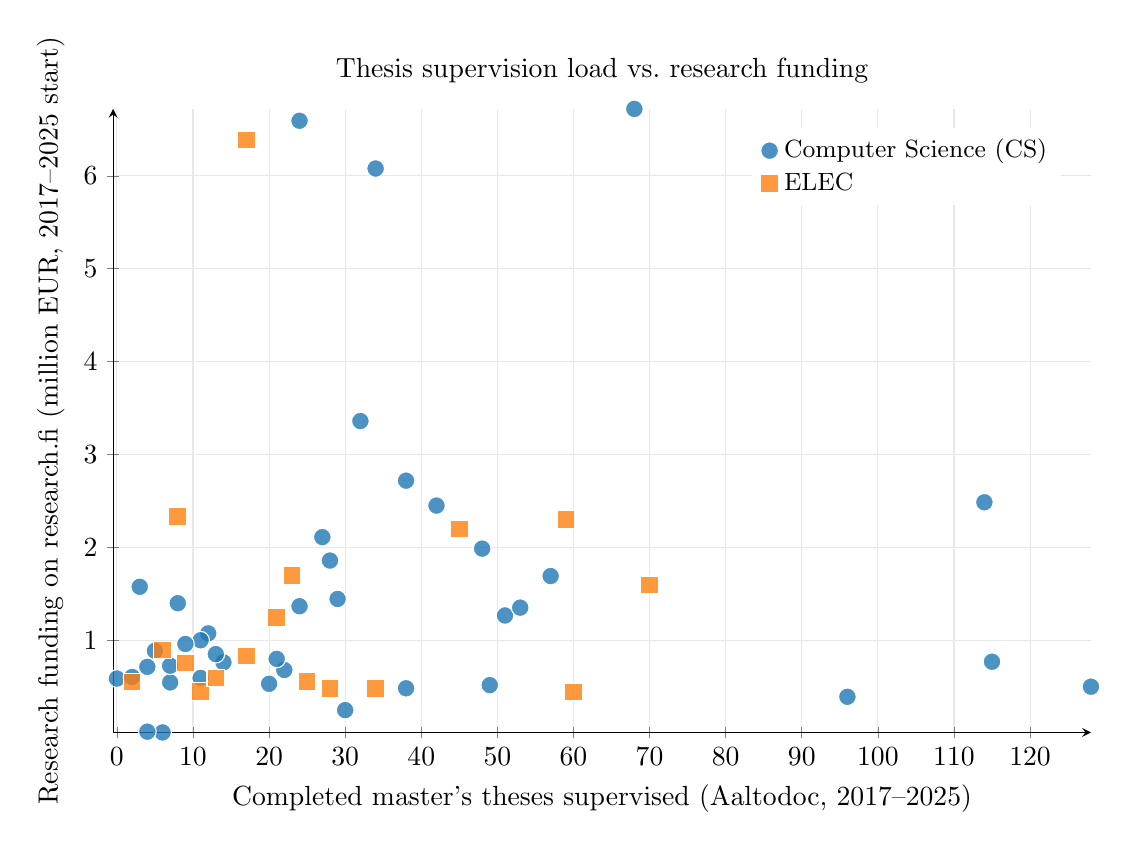
\begin{tikzpicture}
\begin{axis}[
    width=14cm, height=9.5cm,
    xlabel={Completed master's theses supervised (Aaltodoc, 2017–2025)},
    ylabel={Research funding on research.fi (million EUR, 2017–2025 start)},
    title={Thesis supervision load vs.\ research funding},
    grid=both, grid style={gray!18},
    axis lines=left,
    legend pos=north east, legend cell align={left},
    legend style={draw=none, font=\small},
    xmin=-0.5,
]
\addplot[only marks, mark=*, mark size=3.2pt, color=cbBlue, fill=cbBlue, fill opacity=0.8, draw=white, line width=0.4pt] coordinates {
    (20,0.5311) (114,2.4853) (5,0.8863) (6,0.0075) (29,1.4448) (38,0.4830) (7,0.5461) (14,0.7618) (3,1.5757) (49,0.5167) (51,1.2666) (28,1.8580) (12,1.0740) (8,1.3989) (34,6.0783) (22,0.6802) (48,1.9862) (4,0.7138) (57,1.6911) (0,0.5877) (38,2.7179) (24,1.3662) (30,0.2481) (13,0.8509) (53,1.3512) (115,0.7689) (21,0.7997) (42,2.4498) (24,6.5924) (68,6.7199) (4,0.0160) (128,0.5000) (7,0.7257) (32,3.3595) (27,2.1101) (2,0.6043) (11,0.5943) (11,0.9999) (96,0.3916) (9,0.9598)
};
\addlegendentry{Computer Science (CS)}
\addplot[only marks, mark=square*, mark size=3.2pt, color=cbOrange, fill=cbOrange, fill opacity=0.8, draw=white, line width=0.4pt] coordinates {
    (11,0.4505) (17,6.3853) (2,0.5490) (8,2.3353) (45,2.1959) (9,0.7563) (59,2.2981) (28,0.4836) (70,1.5965) (13,0.5941) (60,0.4450) (23,1.6967) (6,0.8960) (25,0.5560) (21,1.2427) (34,0.4797) (17,0.8317)
};
\addlegendentry{ELEC}
\end{axis}
\end{tikzpicture}
\end{document}
